\chapter{Desenvolvimento do Jogo}\label{ch:Desenvolvimento}

%A documentação do jogo é o Game Design Document (ou GDD para os íntimos). Alguns chamam também de Game Design Bible. É a mesma coisa

O processo de desenvolvimento de jogos digitais é uma tarefa que exige do(s) desenvolvedor(es) conhecimentos de programação. Um jogo para ser desenvolvido, deve ser escrito em uma determinada linguagem de programação, o que acaba por obrigar que o(s) desenvolver(es) do jogo tenha(m) conhecimento sobre esta linguagem. Embora existam linguagens de programação visual, o conhecimento sobre lógica de programação ainda é parte fundamental para o desenvolvimento de um jogo. 

%(programação em blocos ou Visual Scripting) : linguagem de programação visual. 

Um jogo digital requer conhecimentos computacionais específicos para o seu desenvolvimento. Os jogos sérios, além de exigirem estes mesmo conhecimentos, devem ser desenvolvidos sobre príncipios pedagógicos e metodológicos de ensino. Sendo assim, a \autoref{sec:motor} descrever os principais aspectos computacionais levados em consideração para o desenvolvimento de um jogo sério voltado para prevenção da violência sexual infantil. Já a \autoref{sec:DN} discorre sobre a estrutura metodologica de ensino e a forma como esta se organiza sobre os níveis do jogo. É fundamental salientar aqui que, embora aspectos artísticos, sonoros, ergonomicos, estéticos e jurídicos sejam importantes no desenvolvimento de jogos, eles não são abordados neste trabalho, assim como questões sobre criptografia e banco de dados.




%Embora importantes no cenário de desenvolvimentos de jogos, aspectos artísticos, sonoros, ergonomicos, estéticos, aspectos jurídicos. 

%criptografia, banco de dados,

%demais aspectos de correspondem a infraestrutura não serão abordadaos. 


\section{Motor de Jogo}\label{sec:motor}

Godot, Unreal, Unity....

%https://pt.wikipedia.org/wiki/Motor_de_jogo
%https://en.wikipedia.org/wiki/List_of_game_engines

Game Engine é um dos componentes mais importantes para o desenvolvimento de jogos por oferecer gerenciamento do fluxo de código, simulação de física e/ou suporte a diferentes plataformas (MACHADO; MORAES; NUNES, 2009), incluem editores de níveis, animação de personagens, pré-visualização do jogo, programação que suporta scripts, ou recursos de arrastar e soltar. Podem ser 2D (GameMaker, Cocos2D, Stencyl, entre outras) ou 3D (Unity3D, UDK, CryEngine, Blender, Panda 3D, entre outras).

A game engine escolhida para desenvolvimento foi a Unity3D, devido licença livre de uso para desenvolvimento de jogos sem fins lucrativos, suporte para multiplataforma, potencial para criação de jogos simples e complexos e recursos integrados.

Unity3D um game engine criado pela Unity Technologies, permite criação de jogos online e off-line. Utiliza o conceito de assets que funciona como um plug-in, onde o usuário pode importar ou apenas copiar o arquivo asset para uma pasta específica. Usa JavaScript, C\# e Boo como as principais linguagens de programação, e uma das vantagens é que pode ser executado em diversas plataformas, incluindo Windows, Mac, Linux e também móvel. As linguagens podem usar as bibliotecas .NET subjacentes que suportam bancos de dados, expressões regulares, XML, acesso a arquivos e networking (WANG et al., 2010).

Permite criação de jogos em 2D ou 3D, uma vez criado o jogo pode ser adaptado a diversas plataformas disponíveis: móveis, VR, desktop, console, plataformas de TV e Web. Suporta os tipos de dispositivos de entrada convencionais usados com jogos (teclado, joypad, etc) mas também telas sensíveis ao toque e capacidade de detecção de movimentos de dispositivos móveis. Pode utilizar também, microfone e webcam para entrada de áudio e vídeo e através de script C\# por exemplo, é possível implementação de conexão serial via USB para entrada e saída de dados. A Unity3D oferece desenvolvimento web sem esforço, processamento em tempo real, sincronização e chamadas remotas de procedimentos.



%\section{Ensinamento}\label{sec:ensinamento}

%Os participantes devem ser capazes de identificar corretamente a localização e o nome das partes do corpo.

%As crianças devem saber diferenciar as partes íntimas do corpo das demais partes. 

%Os participantes devem manifestar competências sobre o uso seguro das tecnologias da informação e comunicação.

%As crianças devem saber reconhecer um adulto em quem possam confiar.

\section{Desenho de Níveis e Ensinamentos}\label{sec:DN}


O estilo de jogo foi aventura, por que esse foi o estilo de jogo com melhor equilibrio entre meninos e meninas %https://content.sciendo.com/view/journals/nor/30/2/article-p69.xml

Primeira fase..

Segunda fase..

Terceira fase..

Quarta fase..


\begin{figure}[htb]
\caption{\label{fig:Diagrama}Diagrama de Atividades do Jogo}
\begin{center}
  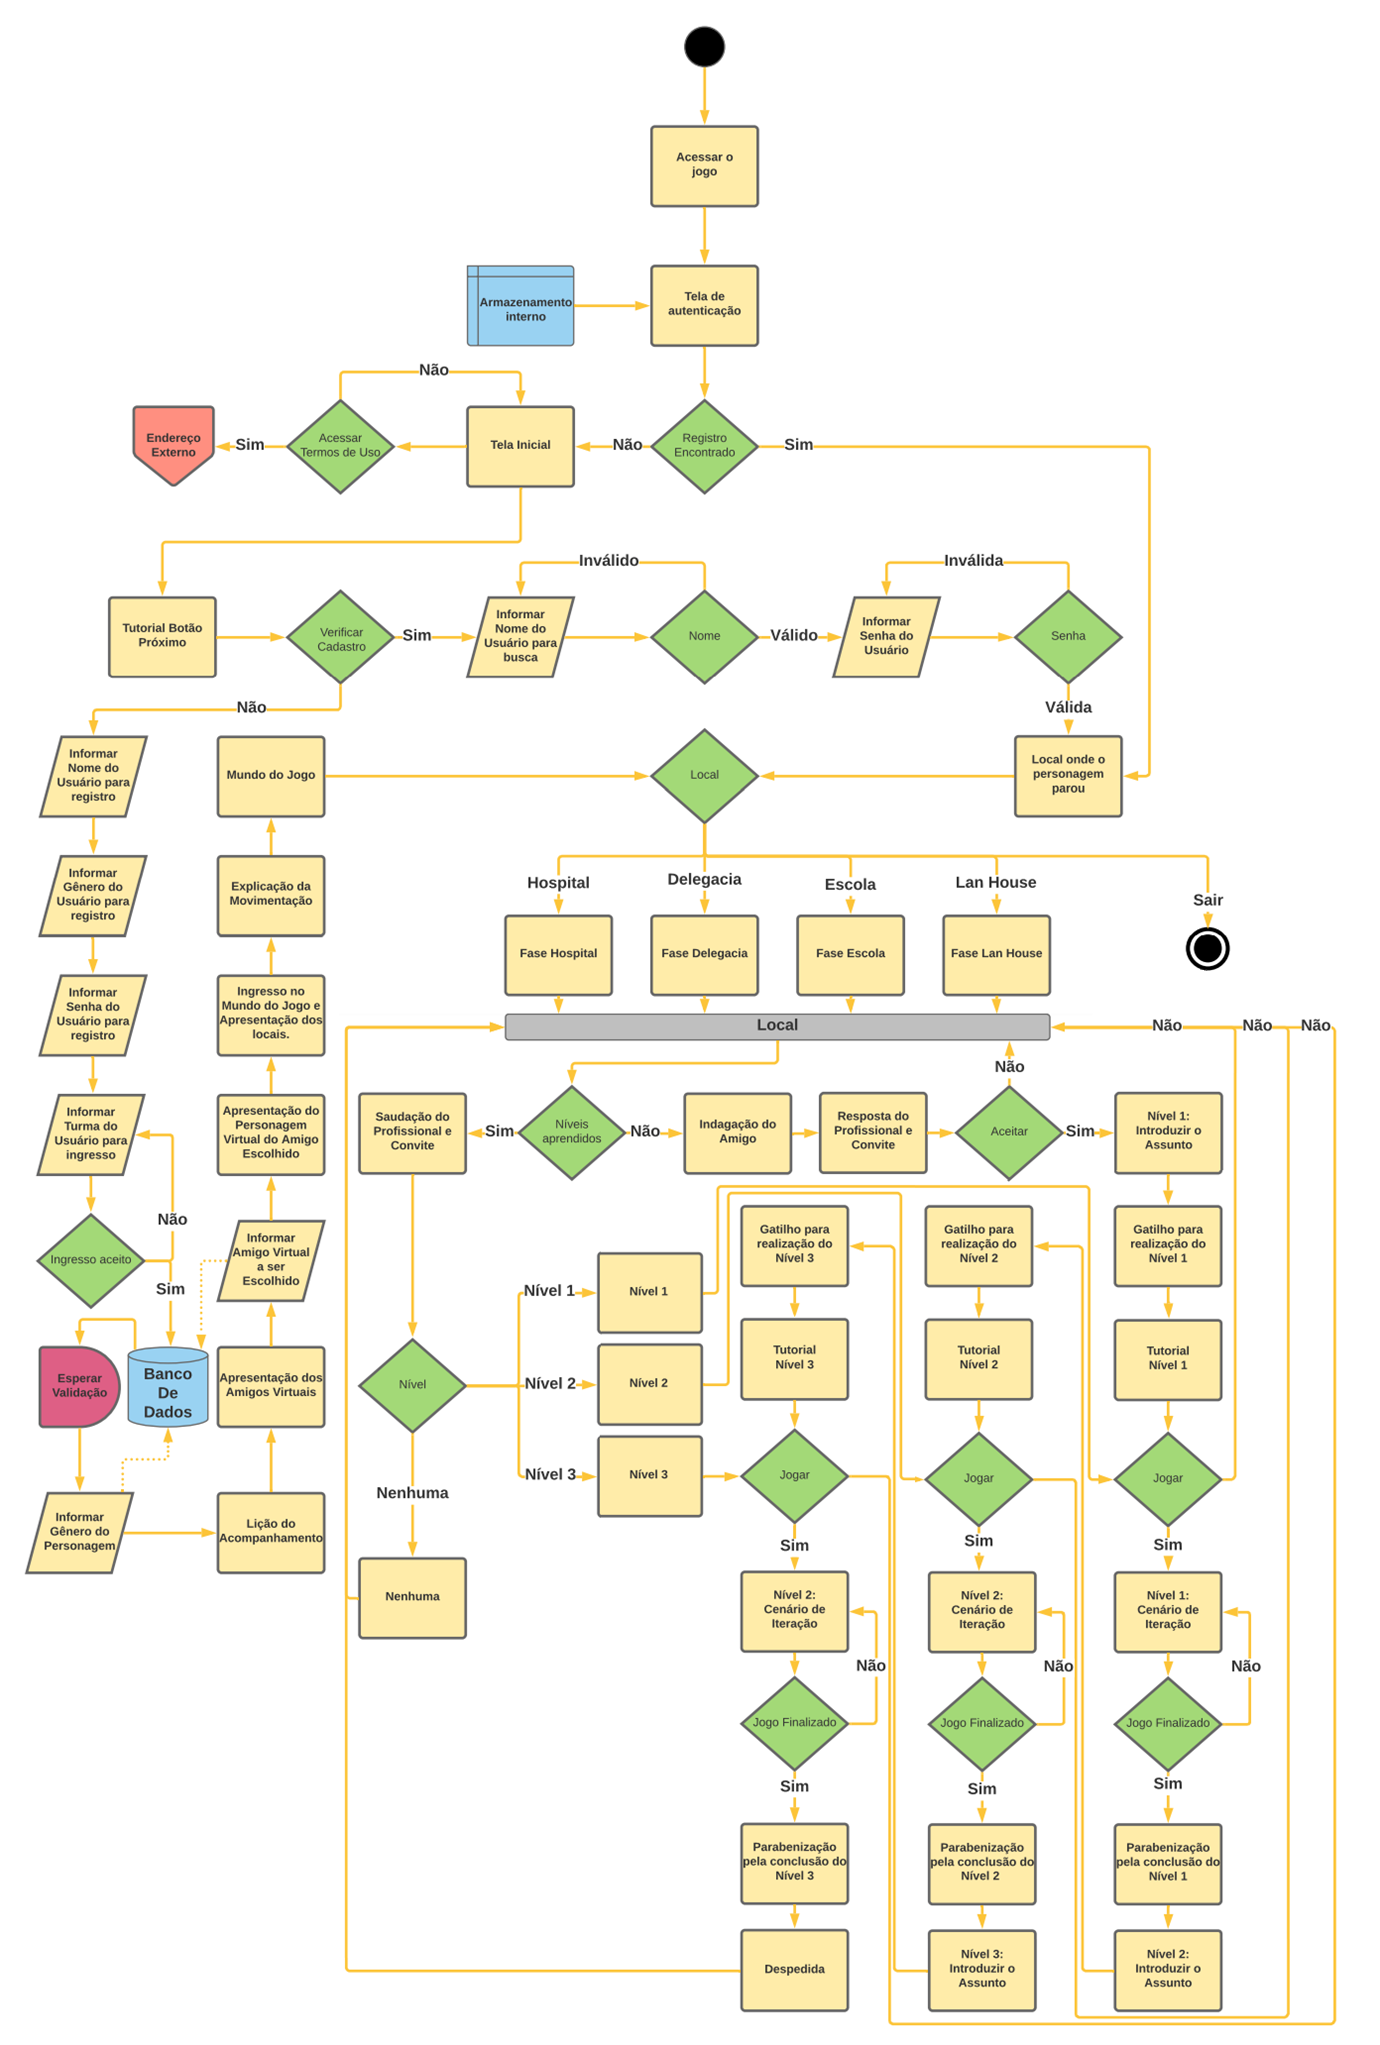
\includegraphics[width=\linewidth]{./Figuras/DiagramaJoginho.png}
  \end{center}
\legend{Fonte: os autores}

\end{figure}






\begin{comment}
propósito

Orientações em Sexualidade

Plataforma

Publico Alvo

Estilo

Estética

Arte

Fonte

Escalabilidade/Flexibilidade

Audio

Musica

Leiaute de Níveis

UX

Gamificação

Ergonomia de Botões

Artefato

Licença

Termos de Serviço

Política de Privacidade

Criptografia

Banco de Dados
\end{comment}

%%%%%%%%%%O enredo é tão importante para jogos sérios como não-sérios, pois permite que o jogador se projete na personagem do jogo (McDaniel et al., 2010). [tese Adilson] = Falar da dinâmica do herói mudo.


%Digital Natives. Our students today are all “native speakers” of the digital language of computers, video games and the Internet. %https://www.marcprensky.com/writing/Prensky%20-%20Digital%20Natives,%20Digital%20Immigrants%20-%20Part1.pdf %https://colegiongeracao.com.br/novageracao/2_intencoes/nativos.pdf


%Para que um game seja completo, e atenda a critérios de usabilidade, é essencial promover algum mecanismo que facilite o aprendizado do funcionamento do jogo. De acordo com Squire et al. (2005, p.41), mediadores são fundamentais nos primeiros dias%https://www.udesc.br/arquivos/cct/id_cpmenu/1024/diego_buchinger__1__15167055468902_1024.pdf


%A Metodologia Institucional “Aprender na Prática”, que prevê “a ação educativa na participação ativa e crítica do aluno em sua aquisição de conhecimentos práticos e teóricos” [UNICSUL, 2004] 